\documentclass{article}
\usepackage[utf8]{inputenc}
\usepackage{subcaption}
\usepackage{amsmath}
\usepackage{amssymb}
\usepackage{tabto}
\usepackage{hyperref}
\usepackage{titlesec}
\usepackage{colortbl}
\usepackage{float}
\usepackage{xcolor, soul}
\usepackage{fancyhdr}
\usepackage{graphicx}
\usepackage{braket}
\usepackage{multirow}
\usepackage{afterpage}
\usepackage{placeins}
\usepackage{booktabs}
\usepackage{array}
\usepackage[rightcaption]{sidecap}
\usepackage{verbatim}
\usepackage{tikz}
\usepackage{algorithm}
\usepackage{algpseudocode}
% \usepackage[caption=false]{subfig}
\sethlcolor{green}
\usepackage [ a4paper, margin = 1in ]{ geometry }
\hypersetup{
    colorlinks=true,
    linkcolor=blue,
    filecolor=magenta,
    urlcolor=cyan,
}
\begin{document}
\title{\Huge \textbf{CS726 - Advanced Machine Learning \\ Programming Assignment 1} }
\author{
\textbf{Saksham Rathi (22B1003)}\\
\textbf{Sharvanee Sonawane (22B0943)}\\
\textbf{Deeksha Dhiwakar (22B0988)}
}
\date{February 2025}
\maketitle\clearpage
\section{Triangulation}
This step is implemented in the function \texttt{triangulate}$\_$\texttt{and}$\_$\texttt{get}$\_$\texttt{cliques}. We first check if the graph is already triangulated, using the function \texttt{whether}$\_$\texttt{triangulated} described below:
\begin{algorithm}
\caption{Check if Graph is already Triangulated}
\begin{algorithmic}[1]

    \State \texttt{cycles} $\gets$ Find all cycles in graph

    \For{each \texttt{cycle} in \texttt{cycles}}
        \If{length of \texttt{cycle} $\ge$ 4}      

            \If{there is no shortcut (vertices connected by non-cycle edge)}                
                \State \textbf{return} False
            \EndIf
        \EndIf
    \EndFor

        \State \textbf{return} \texttt{True}
\end{algorithmic}
\end{algorithm}


If the graph is already triangulated, we directly proceed with extracting the maximal cliques. If the graph is not triangulated, we first triangulate it using the minimum degree heuristic, as described in the pseudocode below:

\begin{algorithm}
\caption{Triangulation Process}
\begin{algorithmic}[1]

    \State \texttt{vertices\_left} $\gets$ Set of all vertices



    \While{\texttt{vertices\_left} is not empty}
        \State \texttt{vertex} $\gets$ Vertex in \texttt{vertices\_left} with minimum degree

        \For{each pair $(i, j)$ of neighbours of \texttt{vertex}}
            \If{the graph does not contain an edge between $i$ and $j$}
                \State Add edge $(i, j)$ to the original graph
            \EndIf
        \EndFor
        \State Remove \texttt{vertex} from \texttt{vertices\_left}

        \State Update graph by removing \texttt{vertex} and updating degrees and edges
    \EndWhile
\end{algorithmic}
\end{algorithm}

The figure below shows the run of the triangulation algorithm on an example graph:

\begin{center}
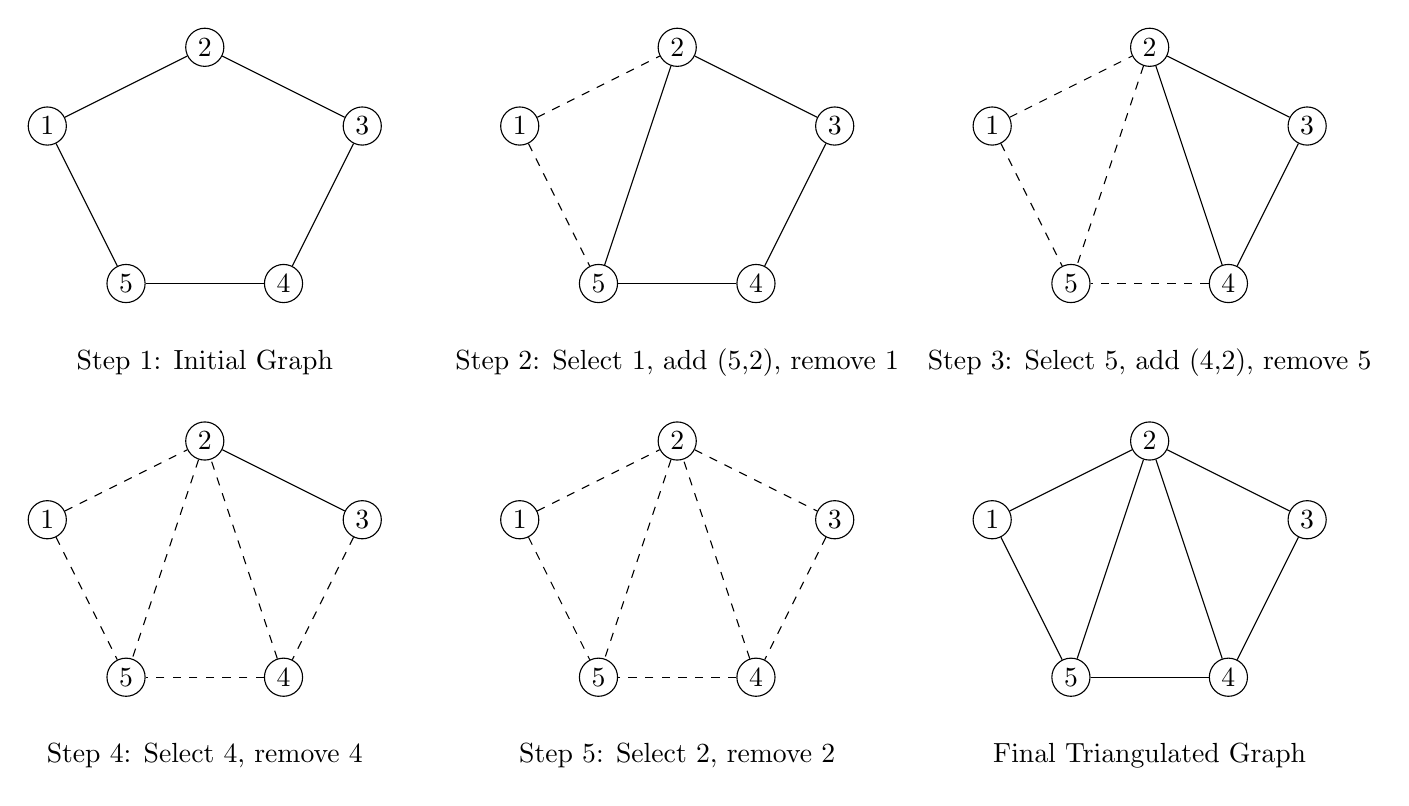
\begin{tikzpicture}[scale=1]

    % Step 1: Initial Graph (First row, first column)
    \begin{scope}
        \node[draw, circle, inner sep=2pt] (1) at (0,2) {1};
        \node[draw, circle, inner sep=2pt] (2) at (2,3) {2};
        \node[draw, circle, inner sep=2pt] (3) at (4,2) {3};
        \node[draw, circle, inner sep=2pt] (4) at (3,0) {4};
        \node[draw, circle, inner sep=2pt] (5) at (1,0) {5};

        \draw (1) -- (2);
        \draw (2) -- (3);
        \draw (3) -- (4);
        \draw (4) -- (5);
        \draw (5) -- (1);

        \node at (2,-1) {Step 1: Initial Graph};
    \end{scope}

    % Step 2: Pick vertex 1, connect 5-2, then remove 1 (First row, second column)
    \begin{scope}[xshift=6cm]
        \node[draw, circle, inner sep=2pt] (1b) at (0,2) {1};
        \node[draw, circle, inner sep=2pt] (2b) at (2,3) {2};
        \node[draw, circle, inner sep=2pt] (3b) at (4,2) {3};
        \node[draw, circle, inner sep=2pt] (4b) at (3,0) {4};
        \node[draw, circle, inner sep=2pt] (5b) at (1,0) {5};

        \draw (2b) -- (3b);
        \draw (3b) -- (4b);
        \draw (4b) -- (5b);
        \draw (5b) -- (2b);
        \draw[dashed] (1b) -- (2b); % Added edge
        \draw[dashed] (1b) -- (5b); % Added edge

        \node at (2,-1) {Step 2: Select 1, add (5,2), remove 1};
    \end{scope}

    % Step 3: Pick vertex 5, connect 4-2, then remove 5 (First row, third column)
    \begin{scope}[xshift=12cm]
        \node[draw, circle, inner sep=2pt] (1b) at (0,2) {1};
        \node[draw, circle, inner sep=2pt] (2b) at (2,3) {2};
        \node[draw, circle, inner sep=2pt] (3b) at (4,2) {3};
        \node[draw, circle, inner sep=2pt] (4b) at (3,0) {4};
        \node[draw, circle, inner sep=2pt] (5b) at (1,0) {5};

        \draw (2b) -- (3b);
        \draw (3b) -- (4b);
        
        \draw (4b) -- (2b);
        \draw[dashed] (1b) -- (2b); % Added edge
        \draw[dashed] (1b) -- (5b); % Added edge
        \draw[dashed] (4b) -- (5b); % Added edge
        \draw[dashed] (2b) -- (5b); % Added edge
        

        \node at (2,-1) {Step 3: Select 5, add (4,2), remove 5};
    \end{scope}

    % Step 4: Pick vertex 4, connect 3-2, then remove 4 (Second row, first column)
    \begin{scope}[yshift=-5cm]
        \node[draw, circle, inner sep=2pt] (1b) at (0,2) {1};
        \node[draw, circle, inner sep=2pt] (2b) at (2,3) {2};
        \node[draw, circle, inner sep=2pt] (3b) at (4,2) {3};
        \node[draw, circle, inner sep=2pt] (4b) at (3,0) {4};
        \node[draw, circle, inner sep=2pt] (5b) at (1,0) {5};

        \draw (2b) -- (3b);
        \draw[dashed] (3b) -- (4b);
        
        \draw[dashed] (4b) -- (2b);
        \draw[dashed] (1b) -- (2b); % Added edge
        \draw[dashed] (1b) -- (5b); % Added edge
        \draw[dashed] (4b) -- (5b); % Added edge
        \draw[dashed] (2b) -- (5b); % Added edge
        

        \node at (2,-1) {Step 4: Select 4, remove 4};
    \end{scope}

    % Step 5: Remove remaining vertices (Second row, second column)
    \begin{scope}[yshift=-5cm, xshift=6cm]
     \node[draw, circle, inner sep=2pt] (1b) at (0,2) {1};
        \node[draw, circle, inner sep=2pt] (2b) at (2,3) {2};
        \node[draw, circle, inner sep=2pt] (3b) at (4,2) {3};
        \node[draw, circle, inner sep=2pt] (4b) at (3,0) {4};
        \node[draw, circle, inner sep=2pt] (5b) at (1,0) {5};

        \draw[dashed] (2b) -- (3b);
        \draw[dashed] (3b) -- (4b);
        
        \draw[dashed] (4b) -- (2b);
        \draw[dashed] (1b) -- (2b); % Added edge
        \draw[dashed] (1b) -- (5b); % Added edge
        \draw[dashed] (4b) -- (5b); % Added edge
        \draw[dashed] (2b) -- (5b); % Added edge
        

        \node at (2,-1) {Step 5: Select 2, remove 2};

    \end{scope}

        \begin{scope}[yshift=-5cm, xshift=12cm]
     \node[draw, circle, inner sep=2pt] (1b) at (0,2) {1};
        \node[draw, circle, inner sep=2pt] (2b) at (2,3) {2};
        \node[draw, circle, inner sep=2pt] (3b) at (4,2) {3};
        \node[draw, circle, inner sep=2pt] (4b) at (3,0) {4};
        \node[draw, circle, inner sep=2pt] (5b) at (1,0) {5};

        \draw(2b) -- (3b);
        \draw (3b) -- (4b);
        
        \draw (4b) -- (2b);
        \draw (1b) -- (2b); % Added edge
        \draw (1b) -- (5b); % Added edge
        \draw (4b) -- (5b); % Added edge
        \draw (2b) -- (5b); % Added edge
        

        \node at (2,-1) {Final Triangulated Graph};

    \end{scope}

    

\end{tikzpicture}
\end{center}
    Once we obtain the triangulated graph, we extract the maximal cliques from it using the function \texttt{get\_maximal\_cliques}, which uses the Bron-Kerbosch algorithm described below:

\begin{algorithm}
\caption{Bron–Kerbosch Algorithm for Finding Maximal Cliques}
\begin{algorithmic}[1]
    \Procedure{Bron\_Kerbosch}{$\text{current\_clique}, \text{candidates}, \text{excluded}, \text{maximal\_cliques}$}
        \If{$\text{candidates}$ is empty \textbf{and} $\text{excluded}$ is empty} 
            \State Add $\text{current\_clique}$ to $\text{maximal\_cliques}$
            \State \Return
        \EndIf
        
        \For{each vertex $v$ in $\text{candidates}$}
            \State \texttt{Bron\_Kerbosch}($\text{current\_clique} \cup \{v\},$
            \State \hspace{1cm} $\text{candidates} \cap \text{Neighbors}(v),$
            \State \hspace{1cm} $\text{excluded} \cap \text{Neighbors}(v),$
            \State \hspace{1cm} $\text{maximal\_cliques}$)
            \State Remove $v$ from $\text{candidates}$
            \State Add $v$ to $\text{excluded}$
        \EndFor
    \EndProcedure
\end{algorithmic}
\end{algorithm}




















\section{Junction Tree Construction}
This step is implemented in the $\texttt{get\_junction\_tree}$ function. We use the maximal cliques obtained after the triangulation process to create the junction tree while maintaining the running intersection property. Each clique in this tree retains its assigned potential values.
\begin{algorithm}
\caption{Constructing a Junction Tree from Maximal Cliques}
\begin{algorithmic}[1]
\Require Set of maximal cliques $\mathcal{C}$
\Ensure Junction tree satisfying the running intersection property

\State Initialize an empty priority queue $T$
\ForAll{pairs $(C_1, C_2)$ in $\mathcal{C}$}
    \State Compute the intersection set $S = C_1 \cap C_2$
    \If{$S \neq \emptyset$}
        \State Compute weight $w = |S|$
        \State Push $(-w, C_1, C_2)$ onto $T$ (negative weight for max heap)
    \EndIf
\EndFor
\\
\State Initialize $parent[C] = C$ and $rank[C] = 0$ for all $C \in \mathcal{C}$
\\
\Function{FindParent}{$C$}
    \If{$parent[C] \neq C$}
        \State $parent[C] \gets \text{FindParent}(parent[C])$
    \EndIf
    \State \Return $parent[C]$
\EndFunction
\\
\Function{Union}{$C_1, C_2$}
    \State $root_1 \gets \text{FindParent}(C_1)$
    \State $root_2 \gets \text{FindParent}(C_2)$
    \If{$root_1 \neq root_2$}
        \If{$rank[root_1] > rank[root_2]$}
            \State $parent[root_2] \gets root_1$
        \ElsIf{$rank[root_2] > rank[root_1]$}
            \State $parent[root_1] \gets root_2$
        \Else
            \State $parent[root_2] \gets root_1$
            \State $rank[root_1] \gets rank[root_1] + 1$
        \EndIf
        \State \Return True
    \EndIf
    \State \Return False
\EndFunction
\\
\State Initialize an empty set $MST$ (Minimum Spanning Tree)
\While{$T$ is not empty}
    \State Pop $(w, C_1, C_2)$ from $T$
    \If{\Call{Union}{$C_1, C_2$}}
        \State Add edge $(C_1, C_2)$ to $MST$
    \EndIf
\EndWhile

\State \Return $MST$
\end{algorithmic}
\end{algorithm}
Consider the given triangulated graph:
\begin{center}
    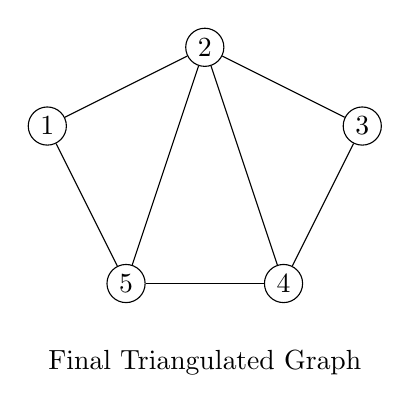
\begin{tikzpicture}
    \begin{scope}[yshift=-5cm, xshift=12cm]
     \node[draw, circle, inner sep=2pt] (1b) at (0,2) {1};
        \node[draw, circle, inner sep=2pt] (2b) at (2,3) {2};
        \node[draw, circle, inner sep=2pt] (3b) at (4,2) {3};
        \node[draw, circle, inner sep=2pt] (4b) at (3,0) {4};
        \node[draw, circle, inner sep=2pt] (5b) at (1,0) {5};

        \draw(2b) -- (3b);
        \draw (3b) -- (4b);
        \draw (4b) -- (2b);
        \draw (1b) -- (2b); 
        \draw (1b) -- (5b);
        \draw (4b) -- (5b);
        \draw (2b) -- (5b); 

        \node at (2,-1) {Final Triangulated Graph};
    \end{scope}
    \end{tikzpicture}
\end{center}
From the triangulated graph, we obtain the maximal cliques:
\[
C_1 = \{1,2,5\}, \quad
C_2 = \{2,3,4\}, \quad
C_3 = \{2,4,5\}, \quad
\]
The intersection sets are as follows: 
\begin{align*}
C_1 \cap C_3 &= \{2,5\}, \quad |C_1 \cap C_3| = 2 \\
C_1 \cap C_2 &= \{2\}, \quad |C_1 \cap C_2| = 1 \\
C_3 \cap C_2 &= \{2,4\}, \quad |C_3 \cap C_2| = 2 \\
\end{align*}
We construct edges with weights corresponding to intersection sizes:
\[
(C_1, C_3, 2), \quad (C_3, C_2, 2), \quad (C_1, C_2, 1)
\]
Using Kruskal’s algorithm:
\begin{enumerate}
    \item Sort edges: $(C_1, C_3, 2)$, $(C_3, C_2, 2)$, $(C_1, C_2, 1)$.
    \item Add $(C_1, C_3)$ (weight 2).
    \item Add $(C_3, C_2)$ (weight 2).
    \item Ignore $(C_1, C_2)$ (weight 1) as it would form a cycle.
\end{enumerate}
\textbf{Final Junction Tree:}
\[
C_1 \leftrightarrow C_3 \leftrightarrow C_2
\]
\begin{center}
    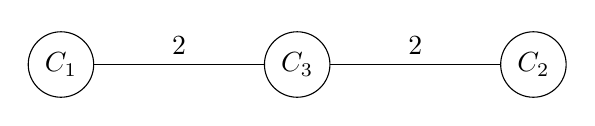
\begin{tikzpicture}
        \node[draw, circle] (C1) at (0,0) {$C_1$};
        \node[draw, circle] (C3) at (3,0) {$C_3$};
        \node[draw, circle] (C2) at (6,0) {$C_2$};

        \draw (C1) -- node[above] {2} (C3);
        \draw (C3) -- node[above] {2} (C2);
    \end{tikzpicture}
\end{center}
For any two cliques $C_i$ and $C_j$ containing the same variable $X$, all cliques along the unique path in the tree must contain $X$. This holds for all intersections.

\clearpage
\section{Marginal Probability}
Here is the pseudocode for sharing messages between the maximal cliques of the graph.\\~\\Firstly, we show how to calculate the Z value for the given graph.

\begin{algorithm}
    \caption{Computation of Partition Function \( Z \)}
    \begin{algorithmic}[1]


    
    \State Arbitrarily root junction tree at \( C_{root} \)

    \State Initialize dicionary \texttt{clique\_depths}
    \State Perform DFS from \( C_{root} \) to populate \texttt{clique\_depths}
    
    \Function{SendMessage}{$C_{from}, C_{to}$}
        \State Compute separator set \( S = C_{from} \cap C_{to} \)
        \State Initialize message vector \( M \) of size \( 2^{|S|} \)
        \State Modify clique potential based on incoming messages
        \For{each state assignment in \( C_{from} \)}
            \State Compute corresponding separator index
            \State Aggregate message value
        \EndFor
        \State Store message \( M(C_{from} \to C_{to}) \)
    \EndFunction
    
    
    \For{each clique from deepest to root}
        \State Send messages to parent cliques
    \EndFor
    
    \For{each clique from root to leaves}
        \State Send messages to child cliques
    \EndFor
    
    \State Compute partition function \( Z \) using root clique potential and received messages
    \State \Return \( Z \)
    
    \end{algorithmic}
\end{algorithm}

Here is the pseudocode for computing the marginal probabilities in the graphical model using message passing.

\begin{algorithm}
    \caption{Computation of Marginal Probabilities}
    \begin{algorithmic}[1]
    

    \State Initialize adjacency list for junction tree
    \State Retrieve partition function $Z$ using previously computed values
    \State Initialize marginal probability list $M$ with zeros

    \For{each variable $X_i$ in the graphical model}
        \State Find a maximal clique $C$ containing $X_i$
        \State Extract the potential function for clique $C$

        \For{each neighboring clique $C'$ of $C$}
            \State Compute separator set $S = C \cap C'$
            \State Retrieve message $M(C' \to C)$
            \For{each assignment in $C$}
                \State Identify corresponding index in $S$
                \State Multiply message values with clique potential
            \EndFor
        \EndFor

        \State Compute marginal probability for $X_i$
        \State Normalize values using $Z$
    \EndFor

    \State \Return $M$
    \end{algorithmic}
\end{algorithm}

\end{document} 